\documentclass[a4paper,12pt]{article}
\usepackage{lmodern}
\usepackage[utf8]{inputenc}
\usepackage{graphicx}
\usepackage{float}
\usepackage{empheq,amsmath}
\usepackage{amstext}
\usepackage{natbib}
\title{Practical Progamming and Numerical Methods \\ Error function}
\author{Marcelo Aron Fetzner Keniger - Studienr.: 201710912}
\usepackage[margin=3cm]{geometry}
\usepackage[pdftex]{hyperref}
\newcommand{\ft}{\footnote}
\newcommand{\tab}[1][1cm]{\hspace*{#1}}
\newcommand*{\figuretitle}[1]{{\centering \textbf{#1} \par \medskip}}
\usepackage{gnuplottex}
\usepackage{enumitem}
\usepackage{cancel}

\begin{document}
\maketitle

\section{Introduction}
\tab The error function, also called Gauss error function, is a special function that occurs in probability, statistics and partial differential equations describing diffusion. It is defined as:

\begin{equation}
    \text{erf(x)} = \frac{1}{\sqrt{\pi}} \int_{-x}^{x} e^{-t^2} dt = \frac{2}{\sqrt{\pi}} \int_{0}^{x} e^{-t^2} dt  
\end{equation}

In statistics, for non-negative values of $x$, for a random variable $Y$ that is normally distributed with mean $0$ and variance $\frac{1}{2}$, the error function describes the probability of $Y$ falling in the range $[-x,x]$. As stated before, the error function also appears in problems involving diffusion. Transient conduction in a semi-infinite solid is governed by the diffusion equations, which has the error function as a solution (depending on the initial conditions, the solution might be the complementary error function, which is nothing more than $1-\text{erf(x)}$).

\section{Assignment}
\tab The given task envolved implementing the error function by integrating numerically, that is, finding the solution, of the differential equation

\begin{equation}
    x'(t) = \frac{2}{\sqrt{\pi}} e^{-t^2}
\end{equation}

with the initial condition $x(0) = 0$. The analitic solution for this equation, with the given initial condition, is precisely the error function. To solve this differential equation numerically, two different methods were used, just for the sake of comparison: the explicit Euler method and the $2^\text{nd}$ order Runge-Kutta method. The program used to apply these methods is shown below in verbatim:

\begin{verbatim}
    program error
  implicit none

  integer x0, tf
  real dt, xex, xanalit, t, pi, x, xaux, fx

!  read*, t, tf, dt

  t = -3
  tf = 3
  dt = 0.01
  x0 = -1
  pi = 3.14159265359

  xex = x0
  x = x0

  do while (t<tf)
     xex = xex +(2/sqrt(pi))*exp(-t**2)*dt

     xanalit = erf(t)

     fx = (2/sqrt(pi))*exp(-t**2)
     xaux = x + (fx*dt)/2

     x = x + fx*dt

     t = t + dt
     
     print*, t, xex, xanalit, x
     
  end do
end program error

\end{verbatim}

In the program above, we calculated the error function in the interval $[-3,3]$ with a step of $0.01$, but these parameters could have easily been defined as command-line arguments with the \textit{read} statement, as shown in the commented line that follows the exclamation point. If that was the case, the parameter $x0$ would also have to be changed, since it is the value of $x$ at the time $t$ ($x(t)$), which is the beginning of our interval. The analytical solution is given by the Fortran intrinsic function erf(x).

\section{Results}
\tab As a final task, we had to plot the error function in the interval calculated. For that, a \textit{Gnuplot} script was made, which will be omitted. The result was the graphic below:

\begin{figure}[H]
\begin{center}
\figuretitle{The error function}
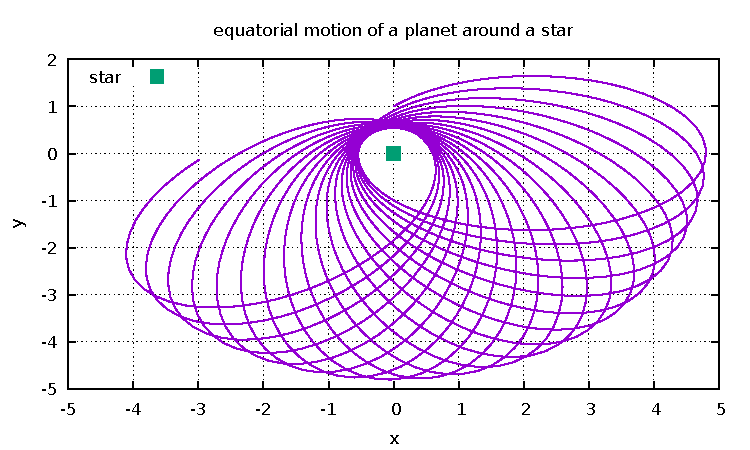
\includegraphics[width=13cm, height=9cm, angle=0]{plot.pdf}
\caption{The error function calculated from the differential equation $(2)$ analyticaly and by two numerical methods.}
\label{fig1}
\end{center}
\end{figure}

As you can see, the numerical methods gave a pretty good approximation to the analytical solution. 

\end{document}
